% 本文是 Science 英文稿的中文逐节对照译稿；英文稿为投稿和科学引文的正式依据。
% 使用 XeLaTeX 编译。翻译不替代英文原稿，不改动原始图像和公式。
\documentclass[UTF8,fontset=fandol,12pt,a4paper]{ctexart}
\usepackage{amsmath,amssymb}
\usepackage{mathptmx}
\usepackage[a4paper,margin=2.35cm]{geometry}
\usepackage{graphicx,array,booktabs}
\usepackage{microtype}
\usepackage[numbers,sort&compress,round]{natbib}
\usepackage[font=small,labelfont=bf,labelsep=period]{caption}
\usepackage[hidelinks,unicode]{hyperref}
\urlstyle{same}
\linespread{1.28}
\setlength{\parindent}{2em}
\setlength{\parskip}{0.35em}
\setlength{\emergencystretch}{1.5em}
\setcounter{topnumber}{4}
\setcounter{bottomnumber}{4}
\setcounter{totalnumber}{6}
\renewcommand{\topfraction}{.95}
\renewcommand{\bottomfraction}{.85}
\renewcommand{\textfraction}{.06}
\renewcommand{\floatpagefraction}{.48}
\setlength{\floatsep}{12pt plus 2pt minus 2pt}
\renewcommand{\citenumfont}[1]{\textit{#1}}
\renewcommand{\bibnumfmt}[1]{#1.}
\setlength{\bibsep}{4pt}
\renewcommand\refname{参考文献与注释}
\newcommand{\dd}{\Delta\theta_t}
\newcommand{\id}{\mathrm{id}}
\newcommand{\PASS}{\textsc{Pass}}
\title{\bfseries 跨神经系统的训练—学习—推理—强化统一动力学}
\author{Mian Wang\\{\small 武汉轻工大学，中国湖北武汉}\\
{\small 通讯作者：\href{mailto:wangmian945@gmail.com}{wangmian945@gmail.com}}}
\date{}
\hypersetup{pdftitle={跨神经系统的训练学习推理强化统一动力学（中文对照译稿）},pdfauthor={Mian Wang}}
\begin{document}
\pagestyle{plain} % 不使用章节名称作为浮动页/声明页的页眉
\maketitle
\begin{center}
{\small\itshape 中文对照译稿，仅供作者审阅；科学引文、正式投稿及术语裁决以英文原稿为准。原始图中的英文标注保持不变。}
\end{center}
\section*{摘要}

尽管神经网络取得了显著成功，但其内部运行机制仍缺乏清晰的科学解释，黑箱问题依然存在。九项 nanoGPT 实验建立了训练—学习—推理（TLI）动力学关系：真实更新引起依赖接收状态的有限幅度功能响应；学习表现为分布式功能支撑的持久重组；目标跨越其特异性读出边界时，才会发生可观察的能力状态转变；推理则在不改变已学习状态的条件下调用这些支撑。第五项实验识别出的因素导出了一种直接预测更新后能力转变的算法，在 5,088 个目标上达到 91.43\% 的准确率和 91.49\% 的四类别宏平均召回率。随后，我们在另外五种神经网络架构中检验了这些关系及其预测。在第七种系统中，集中分配正确反馈削弱了其他已经掌握的技能；重新均衡反馈使这些技能的准确率从 70.31\% 恢复至 99.48\%。将推理产生的后果与后续训练连接起来，便形成统一的训练—学习—推理—强化（TLIR）闭环动力学。

\section{引言}

训练、泛化、能力形成和推理是神经网络研究的核心问题。不同研究领域已经发展出具有重要影响力的理论来研究这些问题。

在\textbf{优化理论}中，神经切线核（Neural Tangent Kernel，NTK）通过网络雅可比矩阵及相应的核，描述特定训练区域内参数变化引起的输出变化 \cite{jacot2018}。边缘稳定性（Edge of Stability）研究训练行为与 Hessian 最大特征值、学习率及损失轨迹之间的关系 \cite{cohen2021}。锐度感知最小化（Sharpness-Aware Minimization，SAM）利用参数邻域内的损失变化构造训练更新，以改善泛化性能 \cite{foret2021}。在这些研究中，\emph{当前状态}由参数及其局部导数或曲率表示；\emph{真实更新}由优化器产生；\emph{响应}则表现为模型输出或损失的变化。

在\textbf{表征学习与泛化}中，频谱偏置（Spectral Bias）考察函数或核模态随频率而异的学习速度 \cite{rahaman2019}。隐式偏置（Implicit Bias）研究优化器为何会选择特定的解，例如可分数据上的最大间隔方向 \cite{soudry2018}。神经坍缩（Neural Collapse）测量类别特征均值、类内变异性和分类器几何结构，揭示训练准确率达到饱和后表征仍可继续变化 \cite{papyan2020}。信息瓶颈（Information Bottleneck）理论研究输入、隐藏表征和目标之间的互信息，包括任务相关信息的保留与压缩 \cite{tishby2015}。这些研究中的\emph{内部组织}表现为频谱模态、优化器选择的解、特征几何或信息结构；\emph{功能变化}则表现为学习速度、解的演化和预测表现的变化。

在\textbf{能力形成}研究中，Grokking 描述了拟合训练样本与取得较强测试泛化能力之间的长时间延迟 \cite{power2022}。后续计算回路研究追踪了这一延迟期间内部计算结构的形成和重组 \cite{nanda2023}。双重下降（Double Descent）研究测试误差如何在接近插值区域时上升，并随模型规模、训练时间或数据条件变化而再次下降 \cite{belkin2019,nakkiran2020}。这些研究利用训练阶段或插值区域表征\emph{当前状态}，利用计算回路与解的演化表征\emph{内部变化}，并通过准确率和泛化误差衡量\emph{可观察能力}。

在\textbf{持续学习}中，灾难性遗忘是指新任务训练降低了先前任务的表现。弹性权重巩固（Elastic Weight Consolidation，EWC）使用先前任务的 Fisher 信息估计参数重要性，并惩罚重要参数的改变 \cite{kirkpatrick2017}。梯度情景记忆（Gradient Episodic Memory，GEM）使用新任务梯度与先前任务梯度的内积约束新任务更新 \cite{lopezpaz2017}。正交梯度下降（Orthogonal Gradient Descent，OGD）则将新梯度投影到能够近似保持先前任务输出的方向 \cite{farajtabar2020}。在这些方法中，\emph{已有状态}包含之前形成的参数和对函数变化敏感的方向；\emph{更新}是受到约束的新任务动作；\emph{相互作用}通过重叠的梯度或功能子空间产生；\emph{能力变化}通过保持、遗忘或迁移进行测量。

在\textbf{推理研究}中，注意力机制（Attention）利用查询（Query）、键（Key）和值（Value）计算依赖输入的信息权重 \cite{vaswani2017}。上下文学习（In-context Learning）研究在模型参数固定时，上下文中的示例和任务信息如何影响预测 \cite{brown2020}。思维链提示（Chain-of-Thought Prompting）研究中间推理步骤如何影响复杂任务表现 \cite{wei2022}。\emph{当前状态}是已训练模型；\emph{输入条件}包括查询、上下文和中间计算；\emph{内部计算}随注意力和激活状态改变；\emph{功能表现}则通过预测结果观察。

在\textbf{强化与反馈驱动训练}中，基于人类反馈的强化学习（Reinforcement Learning from Human Feedback，RLHF）利用偏好和奖励信号调整模型行为 \cite{ouyang2022}。自训练（Self-training）进一步使用模型预测生成训练数据 \cite{xie2020}。递归模型坍塌研究考察连续几代模型使用前代生成的数据进行训练时，低概率模态逐渐丧失的现象 \cite{shumailov2024}。这里，\emph{反馈}由奖励、偏好或生成数据分布提供；\emph{训练动作}是由此产生的更新；随后的\emph{功能变化}通过行为、准确率和生成分布的变化加以观察。

上述研究使用了不同的数学对象——核、Hessian 矩阵、梯度、类别特征、互信息、任务得分、注意力权重与奖励信号——但仍可识别出六类反复出现的共同变量：\emph{当前状态、真实更新、功能响应、内部组织、可观察能力和反馈}。\emph{TLIR 的核心关系是在开展上述跨领域比较之前，通过实验建立的；这里识别这些共同变量，是为了帮助读者理解理论，而不是描述理论最初的发现过程。}

图~\ref{fig:chain} 展示了相互连接的四种动力学角色。

\section{TLI 开环动力学的实验建立}

用于建立 TLI 的九项 nanoGPT 实验，所包含的原生干预、受控对照和独立验证，远比正文所能完整呈现的范围更广。本节概述这些实验的主要发现及由此建立的理论关系。完整实验协议、执行记录、负面结果和独立验证程序均保存在配套仓库中。

\subsection{实验仪器与证据控制}

这些实验所需的仪器，是随着具体测量问题的出现而逐步开发的，并非在理论建立之前就预先假定其存在。

这些仪器共同依托生成事实图（Generation-Fact Graph，GFG），它把记录的模型与优化器状态、真实更新事件、干预、输出及其来源身份连接起来。对于\textbf{训练}，真实更新因果分叉仪器恢复匹配的接收状态，对比完整更新、跳过更新、仅参数更新、优化器记忆变化和双向移植分支，从而区分更新本身与接收该更新的状态的作用。随后，有限幅度响应路径仪器将同一条已记录的真实更新，以预先冻结的不同幅度施加于模型，测量非线性数值响应和离散状态转变。对于\textbf{学习}，CSRG-4C 通过重复基线、单组件门控和双组件门控，测量已注册目标组功能支撑的必要性、备份、替代、协同作用及失效余量。最后，身份对齐目标边界账本把每个注册目标与精确的更新前状态和真实更新相对应，并将响应发生前的记录与更新后正确性的裁决分离。冻结协议、负面对照和独立验证程序进一步约束了对实验结果的解释。


表~\ref{tab:equation_guide} 概述十个编号公式的科学用途和主要符号含义。

\subsection{训练：真实更新与接收状态}

在一个已注册的训练步骤中，参数—优化器状态为 $Z_t=(\theta_t,\omega_t)$，真实参数更新定义为 $\Delta\theta_t=\theta_{t+1}-\theta_t$。

TL-E01 揭示了能力形成、下降和恢复现象，而这些现象不能仅通过损失、准确率或训练步数得到完整刻画。TL-E02 进一步表明，暂停有效的参数—优化器演化会延迟能力形成，而梯度裁剪阈值的对照实验并未复现这一效应。

TL-E03 使用完整更新/跳过更新分支及双向更新移植，建立了如下关系：相同真实更新作用于不同接收状态时，会产生不同的功能响应：
\begin{equation}
 R_q(\theta_A,\Delta\theta_B)\quad\text{vs.}\quad R_q(\theta_B,\Delta\theta_B),
 \label{eq:receiver}
\end{equation}
其中 $R_q(\theta,\Delta)=m_q(\theta+\Delta)-m_q(\theta)$。另行开展的优化器记忆交换检验了历史优化器状态如何影响更新的形成：
\begin{equation}
 \Delta^{(a,b)}=\operatorname{OptStep}(\theta_t,g_t,\omega_{a,b}).
 \label{eq:optmem}
\end{equation}
TL-E04 测量了一次真实更新所产生的完整有限幅度响应：
\begin{equation}
 r_{t,q}(\alpha)=m_q(\theta_t+\alpha\Delta\theta_t)-m_q(\theta_t).
 \label{eq:response}
\end{equation}
实验识别出近线性、饱和、加速、回转和符号反转等响应形式。随后，TL-E05 识别出三类主要响应条件因素：目标边界状态（F1）、目标特异性更新几何（F3）和参数—优化器接收状态（F5）。

\subsection{学习：分布式功能支撑与能力边界}

TL-E06 通过可逆的组件干预，建立了分布式功能支撑的实验证据，包括组件必要性、备份、替代、协同作用和失效余量。

随后，TL-E07 检验了真实训练更新如何持续重组这些支撑：
\begin{equation}
 \Delta P_{t,q}=P_q(\theta_t+\Delta\theta_t)-P_q(\theta_t).
 \label{eq:realloc}
\end{equation}
在 72 个实验区段中，记录了 1,636 次有效的支撑分配转变和 228 次主要支撑组件交接。

TL-E08 通过身份对齐的目标读出边界，将这些内部变化与可观察的能力联系起来。更新前后间隔（margin）的符号用于区分能力保持、丧失、未获得及获得或恢复。因此，学习被界定为\textbf{持久的功能支撑重组}，而能力转变由目标特异性读出边界的跨越决定。

\subsection{推理：冻结状态下对已学习支撑的调用}

INF-E01 研究了 13 条 nanoGPT 训练历史和 52 个检查点。在持久学习状态冻结的条件下，实验测量了依赖查询条件的组件效应、非加性的支撑交互，以及将已训练组件替换为其能力形成前的精确历史版本所产生的变化。

在固定的学习状态 $L^*$ 下，推理调用并组合已经学习形成的支撑：
\begin{equation}
 S_{q,c}^{\mathrm{active}}=\Pi_{q,c}(L^*),\qquad
 y_{q,c}=H_{q,c}(S_{q,c}^{\mathrm{active}}).
 \label{eq:inference}
\end{equation}
组件之间的非加性交互通过下式测量：
\begin{equation}
 I_{ij,q}=f_{\mathrm{full}}-f_{-i}-f_{-j}+f_{-i,-j},
 \label{eq:interaction}
\end{equation}
而对已学习组件版本的依赖通过下式检验：
\begin{equation}
 D_{j,q}=f(q;\theta^*)-f(q;\theta^{(j\leftarrow\mathrm{pre})}).
 \label{eq:rollback}
\end{equation}
精确恢复证明，这些干预并未持续改变已学习状态。实验由此建立了推理的动力学定义：\textbf{推理是在查询条件下调用并组合学习形成的功能支撑，而持久学习状态保持冻结。}

上述九项实验共同建立了相互连接的训练—学习—推理关系，形成 TLI 开环动力学。图~\ref{fig:tlir-evidence} 汇总了 TLIR 四种动力学角色的实验依据。

\section{预测与跨系统验证}

\subsection{由理论导出的目标边界预测}

TL-E05 的响应因素分析确定了三类主要条件因素：当前目标边界状态（F1）、目标特异性更新几何（F3）和参数—优化器接收状态（F5）。这些发现直接导出了 TL-P01 算法，用于预测一次已经形成的真实更新之后，目标的即时边界结果。

对于目标 $y$、竞争目标 $c$ 和隐藏表征 $h$，定义 $b_c=w_y-w_c$ 和 $\Delta b_c=\Delta w_y-\Delta w_c$。利用一阶方向导数 $h'=Dh[\Delta\theta_t]$ 和二阶方向导数 $h''=D^2h[\Delta\theta_t,\Delta\theta_t]$，预测器计算：
\begin{equation}
 \begin{aligned}
 \widehat g_{y,c}={}&b_c^\top h+\Delta b_c^\top h+b_c^\top h'\\
 &+\Delta b_c^\top h'+\tfrac12 b_c^\top h''.
 \end{aligned}
 \label{eq:predict}
\end{equation}
当 $\min_{c\ne y}\widehat g_{y,c}>0$ 时，预测该目标在更新后正确。将预测的更新后正确性与已知的更新前状态结合，即可得到四类能力转变。预测使用的是已经形成的真实更新和响应发生前的信息，\textbf{不读取目标在实际更新后的真实输出}。

\subsection{跨系统验证}

随后，我们在另外五种神经系统中检验了已经建立的 TLI 关系及其预测性结果。表~\ref{tab:systems} 汇总本研究的七种系统，其中第七种 GRU 系统用于单独进行强化反馈实验。

对于另外五种 TLI 系统，分别开展真实更新干预、接收状态比较、有限幅度响应测量、组件联盟功能支撑测量、目标边界结果判定和冻结推理检验。跨系统实现枚举四个注册组件形成的全部 16 种联盟，并计算精确的 Shapley 效应：
\begin{equation}
 \phi_{j,q}=\!\!\sum_{C\subseteq\mathcal C\setminus\{j\}}
 \frac{|C|!(3-|C|)!}{4!}\left[v_q(C\cup\{j\})-v_q(C)\right].
 \label{eq:shapley}
\end{equation}
这里，$v_q(C)$ 表示组件联盟 $C$ 激活时的目标间隔（margin）。

在 ResNet、扩散 U-Net 和 Vision-MoE 中，分别有 42 次、18 次和 36 次参数接收状态交换，其响应差异均超过了预先注册的阈值。各自的目标—更新记录中，有限幅度非线性响应的发生比例分别为 32.23\%、19.25\% 和 35.71\%；功能支撑重分配超过规定阈值的比例则分别为 91.41\%、97.02\% 和 80.43\%。各系统中的冻结推理实验进一步确认了依赖查询条件的功能支撑、非加性交互及对精确训练后组件版本的依赖。

GNN 在三个随机种子中复现了主要 TLI 关系，但其中一个种子未达到预先注册的非线性响应发生频率判据（1.56\%）。硬脉冲 SNN 在四个随机种子中均通过全部 12 项已注册 TLI 判据，从而将证据扩展到具有不连续脉冲动力学的系统。

研究还根据不同任务对方向响应计算作了适配，并在这些系统中评价预测算法。表~\ref{tab:prediction} 给出了更新后即时目标边界分类结果。

预测器在六种 TLI 系统中的五种上取得了较高的四类别宏平均召回率。在硬脉冲 SNN 中，不连续的激活阈值限制了基于局部导数的预测：尽管准确率达到 95.31\%，四类别宏平均召回率仅为 70.74\%。这些实验表明，TLI 核心关系能够跨系统反复出现，同时不同架构在定量功能响应和预测近似方面存在差异。图~\ref{fig:systems} 汇总了六种系统各自的 TLI 实验关系链。

\section{强化：从 TLI 开环动力学到 TLIR 闭环动力学}
\label{sec:reinforcement}

\subsection{由理论导出的反馈动力学预测}

已经建立的 TLI 关系表明，训练会持久重组分布式功能支撑，而推理则调用、组合这些已学习支撑来产生行为。如果推理产生的后果反复反馈到后续训练中，那么由此产生的更新就能进一步重组未来推理所依赖的支撑。

由此得出一项预测：持续、狭窄地集中分配\textbf{正确的正反馈}，可能逐步有利于被强化的能力，同时削弱其他已经掌握的能力。该预测效应来自反馈引导的功能重组，而非错误奖励。

\subsection{实验检验与结果}

RL-E05/E06 在第七种不含注意力机制的共享 GRU 策略网络中检验了这项预测。全部四项技能都在实验分支开始前达到掌握标准。每个分支都从完全相同的参数—AdamW 状态出发；每个完整的两次决策回合仅在正确时获得 $r=1$，否则 $r=0$。

RL-E05 比较了选择性、均衡和冻结反馈。RL-E06 在 3,200 次更新中，每次将 60 个回合分配给四项技能（$q_0,q_1,q_2,q_3$）：均衡组为（15，15，15，15），轻度集中组为（30，10，10，10），高度集中组为（45，5，5，5），独占组为（60，0，0，0）。

RL-E05 观察到相对功能支撑集中、跨技能干扰和依赖组件历史版本的能力权衡，但其预先注册的、更严格的时间先后关系判据\textbf{未能满足}。

在 RL-E06 中，全部 12 个正式随机种子均呈现随反馈集中程度变化的剂量有序效应。被强化技能的平均支撑份额从均衡反馈的 25.54\% 增加到独占反馈的 35.20\%，其他技能的平均间隔则从 9.474 降至 3.962。在轻度和高度集中反馈下，即使准确率尚未下降，其他技能的间隔已开始减小。与均衡反馈相比，独占反馈使其他技能的准确率降低了 39.06 个百分点。

随后，从第 800 次更新时精确的独占反馈状态出发建立两条恢复分支。重新均衡反馈使其他技能的平均准确率从 70.31\% 恢复至 99.48\%，同时将被强化技能保持在 100\%。只训练另外三项技能也使其准确率恢复至 99.83\%，但之前被强化的技能下降至 89.06\%。

这些实验表明，在所测试的共享系统中，正确反馈的分配方式能够重新引导持久功能支撑、改变先前已掌握的能力，并通过反馈重新分配逆转这些变化。

\subsection{TLIR 闭环动力学}

强化把推理产生的后果连接到后续训练动作。由此产生的训练更新重组已学习支撑，进而改变未来推理及其后果。这一反馈闭环将实验建立的 TLI 开环动力学转化为统一的训练—学习—推理—强化（TLIR）闭环动力学。

\section{对正面与负面研究结果的统一解释}
\label{sec:unified}

TLIR首先通过九项nanoGPT实验建立训练、学习、推理之间的动力学关系，再通过跨系统实验与强化反馈实验建立闭环。随后，以同一组接收状态、实际动作、功能响应、支撑重组、能力边界与反馈关系，统一解释已有研究中的正反结果，并从这些关系推导可与独立研究对照的动力学结论。 以下展示8组正反解释与3项理论外推的代表性案例。完整研究包含21组历史正反结果的统一解释和14项理论先行外推，详细分析、数学推导与证据收录于公开证据仓库。

\subsection{正反结果的统一解释}

\noindent\textbf{Sharpness与SAM：参数几何和实际训练效应}\par

正面理论／结果——SAM（Foret等）。 \cite{foret2021} 锐度感知最小化在参数邻域中评估损失扰动，以邻域内的较高损失引导优化方向。在研究所测试的任务中，这种训练动作改善了泛化表现，说明局部敏感性可以成为有效的优化控制量。

反面理论／结果——Sharpness的重参数化反例（Dinh等）。 \cite{dinh2017} 保持神经网络表示函数不变的重参数化可以显著改变原始参数空间中的锐度。因此，相同的输入—输出功能可以对应不同的锐度数值，单独的参数锐度无法唯一决定泛化结果。

TLIR如何统一。 两项研究测量的是动力学链中的不同对象：Sharpness是当前参数状态的局部几何读数；SAM借助该读数改变实际形成的训练动作。动作进入具体接收状态后，引起目标特定的有限幅度功能响应。因而，某个参数空间指标可以随着坐标表示变化，同时依据该指标设计的优化干预仍然可以改变训练结果。核心关系是“局部几何→训练动作形成→接收状态上的功能响应”，而不是“单一几何数值→泛化好坏”。

内部实验锚点。 TL-E03：同一实际更新在不同接收状态下产生不同功能响应；TL-E04：实际更新的有限幅度响应呈现非线性。

\noindent\textbf{NTK与特征学习：固定核动力学和表征演化}\par

正面理论／结果——神经切线核NTK（Jacot等）。 \cite{jacot2018} 在相应无限宽度、惰性训练条件下，网络的输出演化可由固定或近固定的核动力学描述，局部参数变化对功能的作用因而具有可解析的核表示。

反面理论／结果——特征学习参数化（Yang等）。 \cite{yang2021} 在允许实质性特征演化的参数化与训练条件中，内部表征随训练持续改变，网络的后续功能响应需要随之更新，固定核近似不能描述这一过程的全部动力学。

TLIR如何统一。 两者对应接收状态—实际更新—功能响应关系的不同动力学区域：NTK描述功能映射和局部响应变化受限的训练区域；特征学习描述实际更新持续改变内部功能组织、并使后续接收状态发生实质性演化的区域。核动力学与表征学习通过“当前接收状态决定实际更新的响应、更新反过来改变未来接收状态”这一共同关系连接。

内部实验锚点。 TL-E03：功能响应依赖接收状态；TL-E04：有限幅度响应存在非线性；TL-E07：真实更新持续重组功能支撑。

\noindent\textbf{Grokking：迟发能力和提前形成的内部机制}\par

正面理论／结果——Grokking（Power等）。 \cite{power2022} 模型训练准确率已经达到高水平或饱和，测试泛化能力却可能在很长训练延迟后迅速提升，呈现明显的外显能力跃迁。

反面理论／结果——Grokking计算回路研究（Nanda等）。 \cite{nanda2023} 对内部回路的追踪发现，支撑泛化的结构可以在外显测试能力跃迁之前经历持续的形成与重组；能力读出突然变化时，内部学习过程已经持续了一段时间。

TLIR如何统一。 Learning对应功能支撑的持久重组，Capability对应目标功能状态穿过读出边界后的可观察结果。支撑组织可逐步变化，而某个目标的正确性由读出间隔的符号决定；当该间隔跨越零边界时，连续积累的学习表现为离散能力跃迁。两类研究分别观察了同一过程的内部形成轨迹和外部读出时刻。

内部实验锚点。 TL-E06：组件干预揭示分布式功能支撑；TL-E07：真实更新重组支撑；TL-E08：能力转变由目标读出边界决定；TL-P01：预测更新后的目标边界结果。

\noindent\textbf{Neural Collapse：准确率饱和和持续表征形成}\par

正面理论／结果——正确率读出饱和。 当训练样本已被正确分类、训练错误率降至零时，基于正确／错误的离散能力指标达到平台期；在该指标下，后续训练不再增加已正确样本的数量。

反面理论／结果——Neural Collapse（Papyan等）。 \cite{papyan2020} 即使训练误差已经为零，深层特征与分类器仍可持续演化，并形成类内聚集、类别均值几何与分类器方向的特定结构关系。

TLIR如何统一。 正确率只记录目标读出边界的哪一侧；学习记录的是持久的功能组织状态。目标已经被正确分类时，实际训练动作仍可改变目标间隔、组件责任分配与特征几何。因此，同一训练阶段可以同时具有稳定的离散正确率和持续变化的内部功能结构。

内部实验锚点。 TL-E07：能力不变时支撑仍可重组；TL-E08：读出边界决定能力状态；RL-E06：准确率下降前目标间隔已持续变化。

\noindent\textbf{Attention：机制有效性和权重解释争论}\par

正面理论／结果——Attention的计算机制（Vaswani等；Wiegreffe与Pinter）。 \cite{vaswani2017,wiegreffe2019} Attention根据输入内容和查询条件改变信息加权、路由及组合；受控比较也表明，适当构造的注意力解释可以反映某些模型行为机制。

反面理论／结果——Attention权重解释的反例（Jain与Wallace）。 \cite{jain2019} 注意力权重与梯度特征重要性可能不一致；明显不同的注意力权重分布也可能产生相近的最终输出，因而权重数值与完整功能因果作用之间存在可测量的差别。

TLIR如何统一。 冻结的学习状态可以依查询调用不同功能支撑，并通过组件之间的组合产生输出。Attention权重刻画一种瞬时路由和加权关系；完整功能作用则由相应组件及其组合的实际输出效应决定。于是，注意力作为计算机制有效，与单张权重图无法完整表达分布式因果支撑这两个结果可以同时成立。

内部实验锚点。 INF-E01：冻结推理的组件门控、成对干预和版本回滚揭示查询依赖的支撑调用、非加性交互及已学习版本依赖。

\noindent\textbf{RLHF：对齐增益和能力权衡}\par

正面理论／结果——偏好反馈与指令优化（Ouyang等）。 \cite{ouyang2022} 用人类偏好与反馈信号进一步训练模型，可以增强目标指令遵循、偏好一致性及相应任务表现，体现反馈对学习方向的调节作用。

反面理论／结果——Alignment Tax。 同类反馈训练也观察到部分原有基准能力下降；在训练中混入更广泛的预训练分布，可以缓解这些表现退化，说明目标反馈的收益和其他能力的保持存在分配关系。

TLIR如何统一。 反馈改变后续训练样本、奖励与实际更新的分布，实际更新又在共享接收状态中重新配置多项能力的功能支撑。被集中强化的能力获得更多支撑，其他已经掌握的能力可能先损失读出间隔，再发生正确率下降；平衡反馈推动支撑重新分配，使原有能力恢复。正面增益与能力权衡来自同一个反馈—训练—学习闭环。

内部实验锚点。 RL-E06：正确反馈集中造成其他已掌握技能的支撑与能力下降；反馈重新均衡使其恢复。

\noindent\textbf{奖励代理过优化：错误目标绑定和正确反馈过度集中}\par

正面理论／结果——奖励模型与偏好优化。 当真实目标难以直接写成可微训练损失时，奖励模型及偏好信号可以为策略提供可执行的优化方向，促进目标行为形成。

反面理论／结果——Goodhart与奖励过优化。 \cite{gao2023} 奖励模型是实际偏好的代理量；当优化过程逐渐利用代理与真实目标之间的偏差时，代理得分继续改善，真实目标表现却可能下降。

TLIR如何统一。 反馈通过两条具体关系影响实际训练动作。第一条是内容与信用绑定：奖励归属于哪个动作、哪个时间位置，决定优化器收到的训练信号；第二条是反馈分布：即使每个反馈值完全正确，长期集中作用于少数目标也会改变共享功能支撑的分配。代理失配改变了动作的目标绑定；正确反馈过度集中改变了动作的长期分布。两者通过相同的“反馈关系→实际动作→功能支撑与能力”闭环产生不同结果。

内部实验锚点。 RL-E01/E02：反馈绑定与因果信用改变实际训练作用；RL-E06：完全正确但过度集中的反馈也会引起跨技能支撑重分配与能力下降。

\noindent\textbf{Self-training：伪标签学习收益和递归模型坍塌}\par

正面理论／结果——Noisy Student与自训练（Xie等）。 \cite{xie2020} 利用模型产生的伪标签扩展训练数据，再对学生模型进行训练，可以提升ImageNet分类表现及若干稳健性指标，显示生成数据作为反馈输入能够促进学习。

反面理论／结果——递归模型坍塌（Shumailov等）。 \cite{shumailov2024,gerstgrasser2024} 多代模型主要依赖前代生成的数据继续训练时，低概率模式与分布尾部可能逐代消失；持续保留真实数据（Gerstgrasser等）可以改变这种长期信息衰减过程。

TLIR如何统一。 两者共用同一条反馈链：推理输出进入新训练数据，数据组织决定下一轮实际动作，实际动作又改变未来学习状态和推理分布。高质量、多样化伪标签可扩大有效训练信号；递归替换使尾部模式的有效输入持续减少，导致这些模式所依赖的功能支撑不断削弱；持续引入真实数据改变训练输入分布，维持相关模式的学习机会。

内部实验锚点。 TL-E07：训练更新造成持久功能支撑重组；RL-E06：反馈分配改变支撑集中与能力保持，再平衡使能力恢复。

\subsection{理论先行外推与独立研究对照}

理论先行外推从已建立的TLIR关系出发，依次确定动力学变量、数学假设、预测公式与预期结果，再与独立研究进行对照。以下三项分别涉及优化稳定性、能力形成后的持续学习和递归反馈。

\noindent\textbf{演化稳定性：Edge of Stability}\par

TLIR将一次训练写为接收状态与实际动作共同决定的转移：

\[
S_{t+1}=F(S_t,A_t),\qquad A_t=\pi(S_t),
\]

由此得到完整状态演化映射

\[
S_{t+1}=\mathcal F(S_t)=F\bigl(S_t,\pi(S_t)\bigr).
\]

沿该映射的局部稳定性由其雅可比矩阵决定，边缘稳定区域对应\(\rho(D\mathcal F(S_t))\approx 1\)。对于普通梯度下降、局部二次损失和冻结的Hessian，参数更新映射的雅可比为

\[
J_t=I-\eta H_t.
\]

沿正曲率特征方向，局部收缩条件为

\[
|1-\eta\lambda_i|<1,
\qquad \lambda_{\max}=\frac{2}{\eta}
\quad\text{对应边缘阈值}.
\]

这一阈值对应当前接收状态下的局部参数动力学。真实训练在一次有限更新之后，同时改变参数、曲率、优化器记忆和后续的功能响应，因此长期轨迹由连续变化的状态映射决定。由此推得：训练可以在短时越过冻结的局部稳定边界后，通过曲率及接收状态的再组织重新接近稳定区域；带动量与自适应预条件的优化器则具有由联合参数—优化器状态决定的边界。

独立研究中的对应结果包括： \cite{cohen2021,lewkowycz2020,damian2023,cohen2022adaptive}Cohen等观察到神经网络训练长期运行于Hessian边缘稳定区域；Lewkowycz等的catapult机制展示了高学习率下曲率重组与重新收敛；Damian等给出边缘稳定性中的自稳定机制；Cohen等关于自适应优化器的研究进一步揭示了预条件Hessian和优化器状态对稳定边界的作用。

内部实验锚点。 TL-E03：实际更新响应依赖接收状态；TL-E04：有限幅度响应呈非线性；TL-E05：边界、更新几何和接收状态共同影响响应。

\noindent\textbf{能力形成后的持续学习：Implicit Bias与最大间隔}\par

TLIR将能力形成对应于目标读出边界的跨越，将Learning对应于此后仍可继续的持久功能重组。考虑线性可分的二分类任务，目标间隔为

\[
m_i=y_iw^\top x_i.
\]

当所有\(m_i>0\)时，样本已经被正确分类；对于具有指数尾的logistic损失，梯度仍对边界附近的样本赋予更大的权重：

\[
-\nabla L(w)\propto\sum_i y_i x_i e^{-m_i}.
\]

令\(w=ru\)、\(\|u\|=1\)，以及\(\gamma_i(u)=y_i u^\top x_i\)。当\(r\)增大时，

\[
L(w)\approx\sum_i e^{-r\gamma_i(u)},
\]

其主导项来自归一化间隔最小的样本。沿持续降低损失的训练方向，长期组织趋向最大间隔问题：

\[
\max_{\|u\|=1}\min_i y_i u^\top x_i.
\]

在相应的指数尾损失与渐近方向条件下，参数尺度具有对数增长形式：

\[
r(t)\sim\frac{1}{\gamma^\star}\log t.
\]

因此，可观察正确性达到稳定状态之后，实际训练动作仍继续改变参数方向、目标间隔和内部功能组织。Soudry等给出了 \cite{soudry2018,nacson2019,ji2019,gunasekar2018,lyu2020}线性可分logistic回归的最大间隔收敛定理；Nacson、Ji等研究揭示损失尾部对最终隐式组织的选择作用；Gunasekar等展示了优化几何改变隐式偏置的方式；Lyu与Li进一步研究了齐次神经网络中的间隔最大化行为。这些结果共同对应TLIR的“实际动作—持续学习—读出边界”关系。

内部实验锚点。 TL-E07：真实更新持续重组支撑；TL-E08：能力转变取决于读出边界；RL-E06：已掌握能力的平台期仍存在支撑与间隔变化。

\noindent\textbf{递归反馈的信息收缩与真实数据锚定}\par

TLIR闭环将当前推理产生的数据或反馈再次送入训练。设某一低概率信息模式在第\(t\)代有效训练分布中的占比为\(q_t\)，模型生成数据对该模式的平均保留率满足\(0<\rho<1\)。当后续数据完全来自前一代模型时，

\[
q_{t+1}=\rho q_t,
\qquad q_t=q_0\rho^t\longrightarrow 0.
\]

这给出了递归替换条件下低概率模式持续衰减的动力学关系。若每一代有比例\(\alpha\)的真实数据参与训练，且该模式在真实数据中的占比为\(q_{\mathrm{real}}>0\)，则递推变为

\begin{equation}
 q_{t+1}=(1-\alpha)\rho q_t+\alpha q_{\rm real}.
 \label{eq:feedback}
\end{equation}

在\(\alpha>0\)时，该递推趋向非零固定点：

\[
q^\star=\frac{\alpha q_{\mathrm{real}}}
{1-(1-\alpha)\rho}>0.
\]

两种数据组织方式由此产生不同的长期结果：纯递归替换导致尾部模式逐代收缩，持续真实数据输入为该模式提供稳定的信息来源。Shumailov等关于递归模型坍塌的研究观察到尾部模式的优先丢失；Gerstgrasser等和Fu等关于真实数据保留与混合的研究则给出了改变递归退化趋势的实验与理论结果。两组结果共同呈现了反馈分布决定持续学习方向的TLIR闭环机制。 \cite{shumailov2024,gerstgrasser2024,fu2024}

内部实验锚点。 RL-E01：反馈绑定影响实际更新；RL-E06：反馈分配与持续时间改变支撑和能力；TL-E07：训练动作引起持久支撑重组。

欢迎审稿人和其他独立研究者继续由TLIR推导并检验新的预测。

\section{结论}

通过跨神经系统的系统性实验，本研究揭示了贯穿神经网络训练、学习、推理和强化过程的动力学关系。从能力形成与使用到能力丧失与恢复，TLIR 在可观察性能变化与内部功能支撑的组织及其演化之间，建立了能够通过实验检验的因果联系。因此，神经网络能力演化不再只是一种黑箱性能现象，而成为能够通过精确实验干预和定量预测加以研究的动力学过程。

\clearpage
\begin{figure}[!htbp]
 \centering
 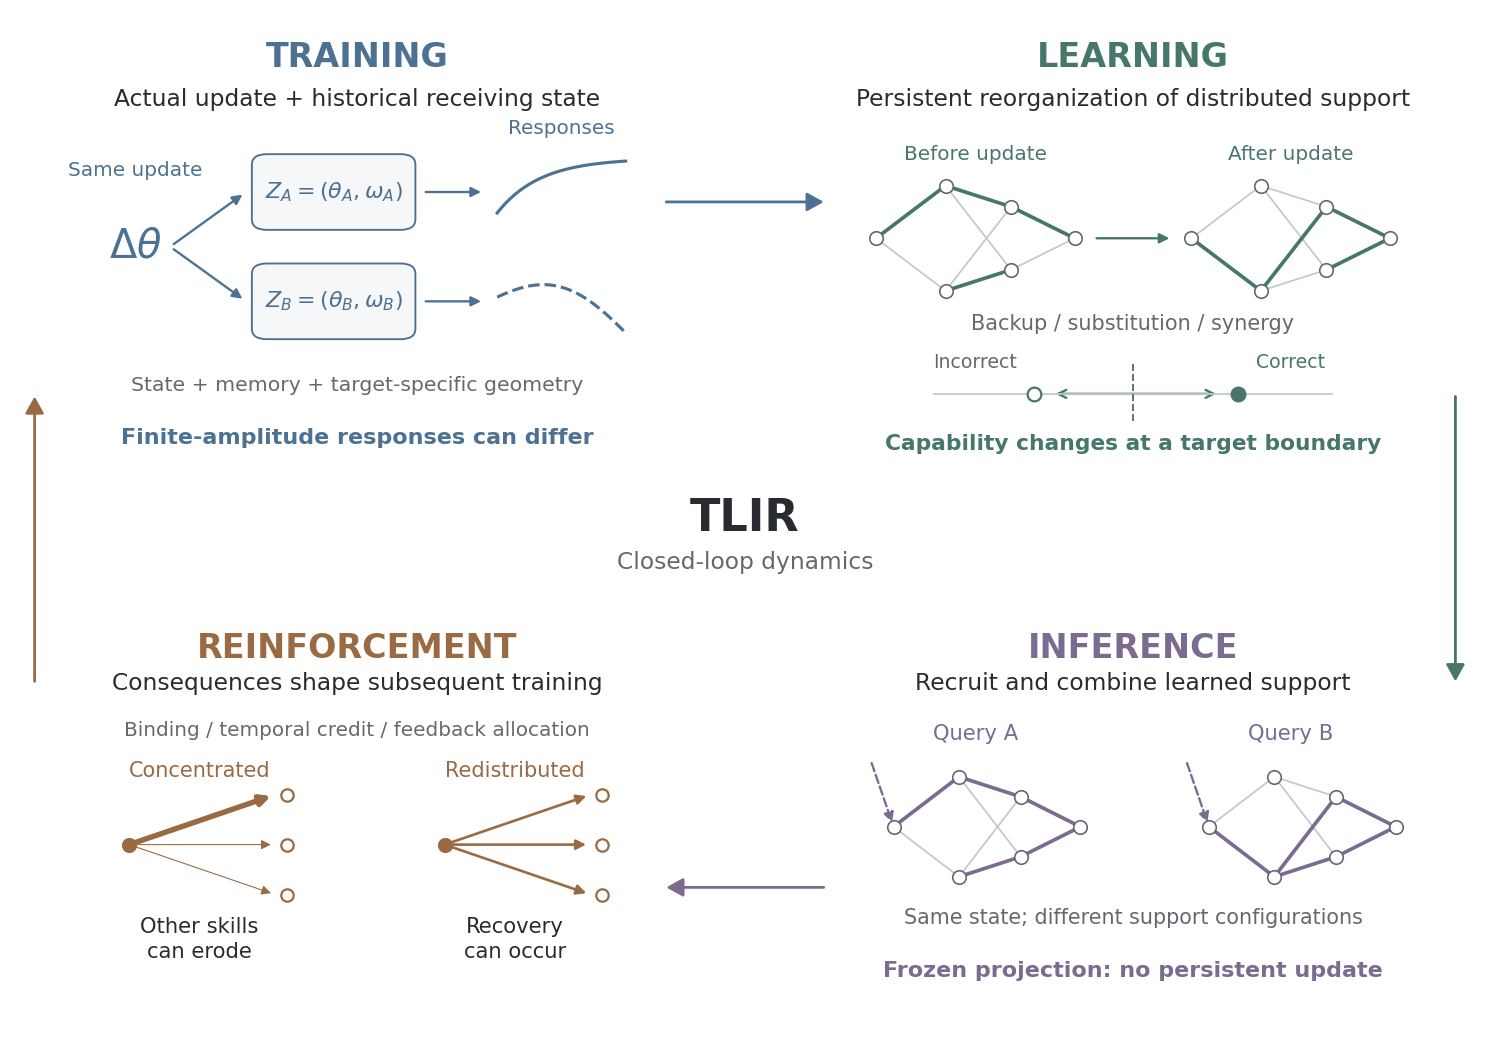
\includegraphics[width=.98\textwidth]{../figures/figure1_tlir_closed_loop.png}
 \caption{TLIR 闭环动力学。训练、学习和推理构成开环核心；强化则将模型行为产生的后果反馈至后续训练，从而形成闭环。}
 \label{fig:chain}
\end{figure}

\begin{figure}[!htbp]
 \centering
 \captionsetup{font=footnotesize}
 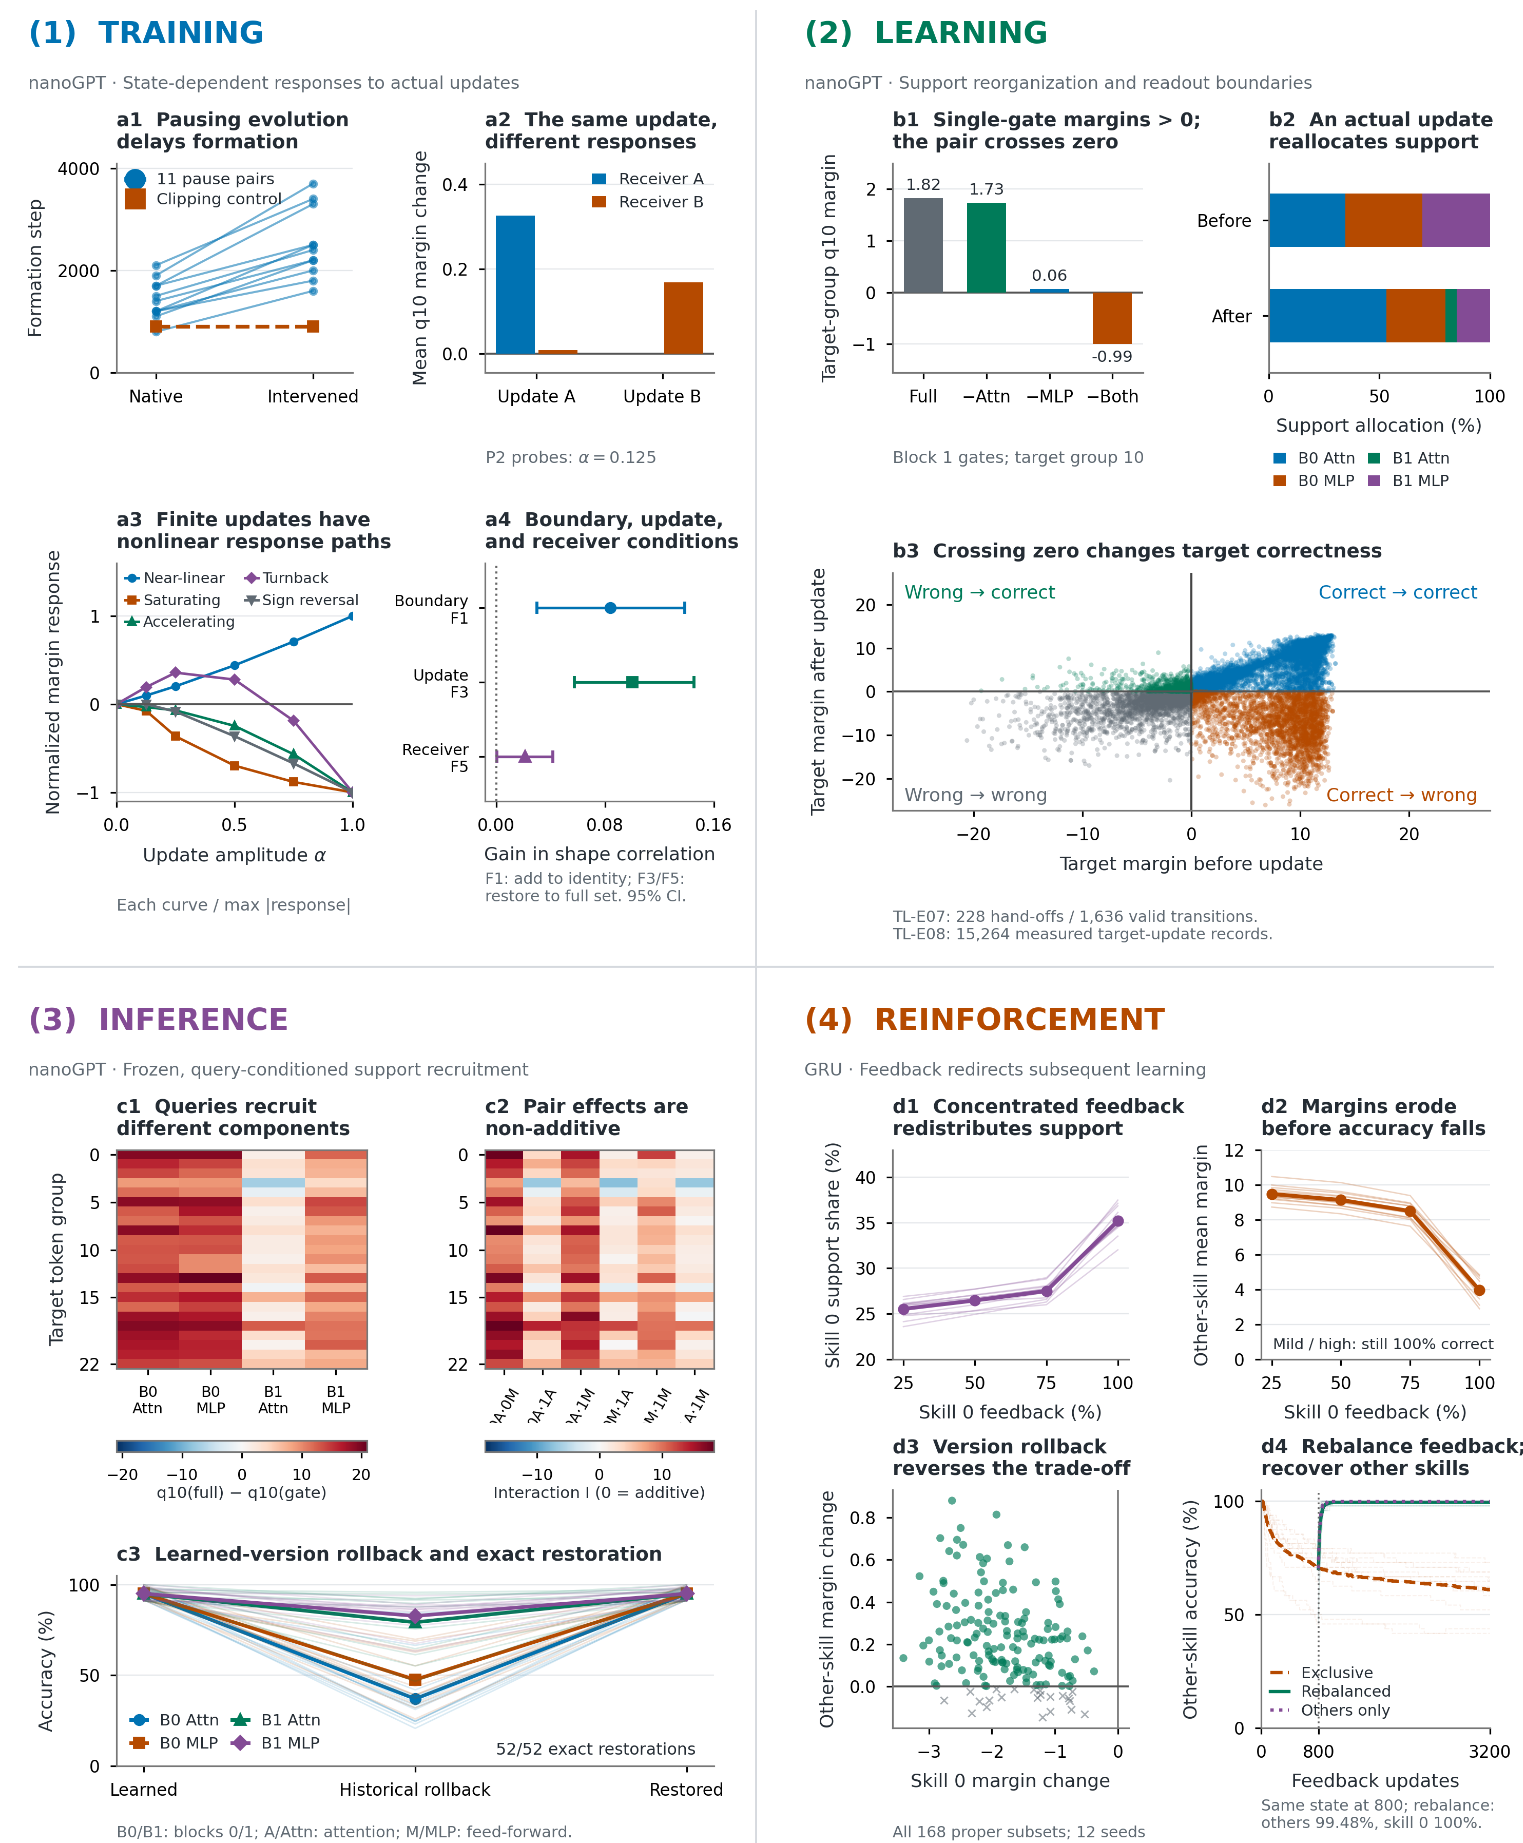
\includegraphics[width=1.00\textwidth,height=.63\textheight,keepaspectratio]{../figures/figure2_experimental_14panel.png}
 \caption{nanoGPT 中训练、学习和冻结推理的代表性实验证据，以及共享 GRU 中反馈驱动的能力变化与恢复。
 (a1) 暂停演化延迟能力形成；
 (a2) 相同真实更新在不同接收状态下引起不同响应；
 (a3) 有限幅度响应的不同类型；
 (a4) 边界、更新和接收状态三类条件因素。
 (b1) 联合移除组件导致目标跨越边界；
 (b2) 一次真实更新引起功能支撑重新分配；
 (b3) 更新前后的目标间隔。
 (c1) 查询条件依赖的组件效应；
 (c2) 非加性成对交互；
 (c3) 已学习组件版本回退与精确恢复。
 (d1) 反馈剂量下的支撑重分配；
 (d2) 准确率下降前的间隔侵蚀；
 (d3) 回退引起的能力权衡；
 (d4) 反馈重新均衡及能力恢复。}
 \label{fig:tlir-evidence}
\end{figure}

\begin{figure}[!htbp]
 \centering
 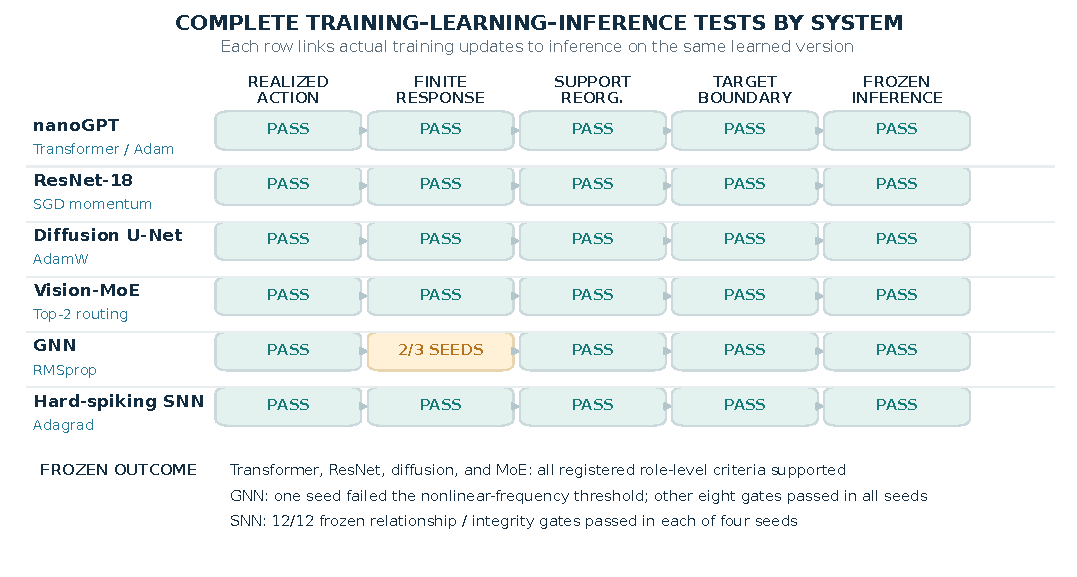
\includegraphics[width=.98\textwidth]{../figures/figure2_six_system_evidence.pdf}
 \caption{六种神经系统各自内部的训练—学习—推理实验关系链。GNN 中有一个随机种子满足九项注册判据中的八项，其非线性响应发生频率低于规定阈值；SNN 在四个随机种子中全部通过十二项注册判据。}
 \label{fig:systems}
\end{figure}

\begin{table}[!htbp]
\caption{七种神经系统：六条 TLI 实验链及一项 GRU 反馈研究。}
\label{tab:systems}
\centering\small\setlength{\tabcolsep}{3pt}\renewcommand{\arraystretch}{1.20}
\begin{tabular}{@{}>{\raggedright\arraybackslash}p{.43\columnwidth}>{\raggedright\arraybackslash}p{.53\columnwidth}@{}}
\toprule
系统（优化器） & 任务／注册组件\\
\midrule
nanoGPT（Adam） & 循环式下一词元预测；4 个注意力／MLP 分支\\
ResNet-18（SGD momentum） & CIFAR-100 分类；4 个残差阶段\\
Diffusion U-Net（AdamW） & CIFAR-10 去噪；4 条 U-Net 路径\\
Vision-MoE（AdamW） & CIFAR-100 分类；4 个路由专家\\
GNN（RMSprop） & 图可达性判断；4 个消息传递模块\\
Spiking SNN（Adagrad） & $8\times8$ 数字图像；4 个脉冲模块\\
GRU（RL-E05/E06；AdamW） & 四技能反馈；4 个共享隐藏状态组\\
\bottomrule
\end{tabular}
\end{table}

\begin{table}[!htbp]
\caption{更新后目标边界分类结果。宏平均召回率为四种实际观察到的能力转变类别的平均召回率；仅有较高准确率并不足以说明预测性能。各系统的预测方法细节与评价集合有所不同。}
\label{tab:prediction}
\centering\small\setlength{\tabcolsep}{4.2pt}\renewcommand{\arraystretch}{1.15}
\begin{tabular}{@{}lrr@{}}
\toprule
系统 & 准确率（\%） & 四类别宏平均召回率（\%）\\
\midrule
nanoGPT & 91.43 & 91.49\\
ResNet-18 & 99.28 & 97.99\\
Diffusion U-Net & 99.60 & 97.98\\
Vision-MoE & 99.63 & 96.95\\
GNN$^{a}$ & 98.54 & 98.62\\
Hard-spiking SNN$^{a}$ & 95.31 & 70.74\\
\bottomrule
\multicolumn{3}{@{}p{.94\columnwidth}@{}}{\footnotesize $^{a}$ GNN 与 SNN 的独立预测检验使用已注册的训练历史。}\\
\end{tabular}
\end{table}

\begin{table}[!htbp]
\caption{RL-E06 每次更新中分配给四项能力的反馈回合数。}
\label{tab:dose}
\centering\small\setlength{\tabcolsep}{4.1pt}\renewcommand{\arraystretch}{1.13}
\begin{tabular}{@{}lrrrr@{}}\toprule
反馈方式 & $q_0$ & $q_1$ & $q_2$ & $q_3$\\\midrule
均衡（Balanced） & 15 & 15 & 15 & 15\\
轻度集中（Mild） & 30 & 10 & 10 & 10\\
高度集中（High） & 45 & 5 & 5 & 5\\
独占（Exclusive） & 60 & 0 & 0 & 0\\\bottomrule
\end{tabular}
\end{table}

\newpage
\input{../references.bbl}

\section*{投稿声明}

\noindent\textbf{资金支持。}
本研究未获得任何资金资助。

\noindent\textbf{作者贡献。}
Mian Wang 提出研究构想；建立原子生成事实模型、生成事实图（GFG）、基于 GFG 的递归科学研究过程，以及训练—学习—推理—强化统一理论；确定科学问题、研究边界与决策标准；提出主要理论假设和概念转换；主导研究计划；分析并解释经过验证的结果；提出前瞻性预测和理论推导；制作图表；撰写并修改论文。

\noindent\textbf{利益冲突。}
作者声明不存在利益冲突。

\noindent\textbf{数据、代码与材料可用性。}
本研究的公开证据仓库按照论文的科学主张组织，旨在支持快速机器辅助审计（\url{https://github.com/wind342/tlir-research-evidence/tree/codex/tlir-paper-evidence-navigation-v1}）。论文—证据映射将主要科学主张、实验、图中子图和报告结果，与冻结协议、源代码、结果记录、来源及校验和清单、独立验证程序建立对应关系。公开证据矩阵还说明了哪些结果能够独立重新计算，以及哪些底层检查点或运行材料没有包含在公开发布的版本中。

\noindent\textbf{生成式人工智能的使用与贡献。}
包括 OpenAI Codex 和 ChatGPT 在内的通用 AI 系统，在基于 GFG 的递归科学研究过程中充当科研代理。在作者的指导下，这些 AI 系统\textbf{发明并实现了四套实验仪器}——CSRG-4C、真实更新因果分叉仪器、有限幅度更新路径仪器和身份对齐目标边界账本——并且设计、实现、启动、监控和执行了论文报告的实验。AI 系统开展了分析、因果干预、匹配重放、反例搜索和独立验证，并参与论文起草、编辑和 LaTeX 排版。所有报告的数值结果均由记录在案的原生程序与执行环境产生，而非 AI 模型直接生成的文本。作者确定科学问题、研究边界和决策标准，审查经过验证的证据，并对科学主张与结果承担责任。

\end{document}
